\section{Software Design Konzepte}
Eine solide Softwarearchitektur ist entscheidend für die erfolgreiche Entwicklung und Wartung eines Programmes. Sie legt den Grundstein für die anschließende Implementierung. Durch eine gute Architektur wird sichergestellt das Programm Skalierbar, Effizient, robust und gut zu warten ist.\\
Hierbei bieten sogenannte Design Patterns Abhilfe. \textit{Jedes Muster beschreibt zunächst ein in unserer Umwelt immer wieder auftretendes Problem, beschreibt dann den Kern der Lösung dieses Problems, und zwar sodass man diese Lösung millionenfach anwenden kann, ohne sich je zu wiederholen} (Christof Alexander \textit{Eine Muster-Sprache} [Löcker verlag, Wien, 1995, Seite x]). Diese Definition für muster bezieht sich auch auf objektorientierte Design Patterns. Das Verwenden dieser Patterns ermöglicht Entwicklern von der Erfahrung anderer zu profitieren, um bereits gelöste Probleme nicht nochmal lösen zu müssen. Zudem steigern sie auch die Codequalität. Der Code wird lesbarer und die Wartung dessen wird leichter. Zudem wird auch die Implementierung neuer Erweiterungen und das Eindenken in die Software durch gängige Designpatterns erleichtert. \cite[S.25 ff]{DesignPatterns}\\
\textit{Alle gut strukturierten objektorientierten Architekturen basieren auf Mustern} (Grady Booch \cite[S.21]{DesignPatterns}).
In den folgenden Kapiteln wird genauer auf die in dieser Arbeit verwendeten Design Patterns eingegangen.      

\subsection{Adapter Pattern}\label{sec:AdapterPattern}
Zweck des Adapter Patterns ist die Anpassung der Schnittstelle einer Klasse an eine andere von dem Client erwarteten Schnittstelle. Somit ermöglicht das Pattern die Zusammenarbeit von zwei Klassen, welche aufgrund ihrer Schnellen nicht möglich wäre. Das Adapter Patern ist auch unter dem Namen Wrapper bekannt, welcher im folgenden Verlauf der Arbeit verwendet wird.\\
Das Pattern kommt immer dann zum Einsatz, wenn eine bereits existierende Klasse genutzt werden soll, jedoch die Schnittstelle der Klasse nicht mit den aktuellen Anforderungen des Clients übereinstimmt. Des Weiteren wird das Pattern verwendet, wenn eine wiederverwendbare Klasse erzeugt werden soll, welche mit unabhängigen und nicht vorhersehbaren Klassen interagieren soll.\\      
\begin{center}
    \begin{figure}[h]
     \centering
     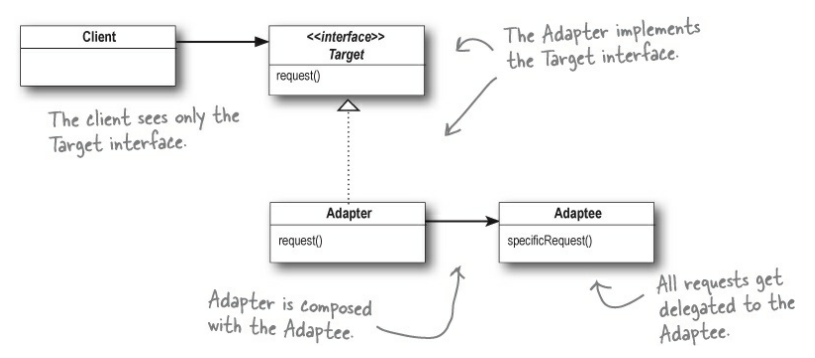
\includegraphics[width=0.6\linewidth]{UMLAdapterPattern}
     \caption{Adapter Pattern Struktur \cite{DesignPatterns}}
    \label{fig:AdapterPattern}
    \end{figure}
\end{center}
\vspace{-2cm}
Das Design Pattern besteht aus einem \textit{Target}, welches die vom Client verwendete Schnittstelle definiert. Zudem kommt der \textit{Client}, welcher mit den Objekten zusammen arbeitet, die der Zielschnittstelle entsprechen. Zuletzt beinhaltet das Adapter Pattern einen \textit{Adaptee} so wie den \textit{Adapter} selbst. Der \textit{Adaptee} definiert eine bestehende Schnittstelle, welche vom \textit{Adapter} adaptiert werden muss.\\ 
Der \textit{Client} ruft die gewünschte Operation auf einer \textit{Adapter}-Instanz auf, welche anschließend die gewünschten \textit{Adaptee}-Operation ausführt.

\subsection{Strategie Design Pattern}\label{sec:StrategyPattern}
Zweck des Strategy (Strategie) Patterns ist es, eine Familie von einzelnen gekapselten und austauschbaren Algorithmen zu schaffen. Dieses Patern ermöglicht eine variable und vom Client unabhängige Nutzung des Algorithmus.\\
Das Pattern kommt zum Einsatz, wenn eine Reihe von zusammenhängenden Klassen sich nur in Ihrem Verhalten unterscheiden, verschiedene Varianten eines Algorithmus erfordert werden, der Client keine Kenntnis von den vom Algorithmus verwendeten Daten haben soll, oder eine Klasse verschiedene Verhaltensweisen aufweist.\\
\begin{center}
    \begin{figure}[h]
     \centering
     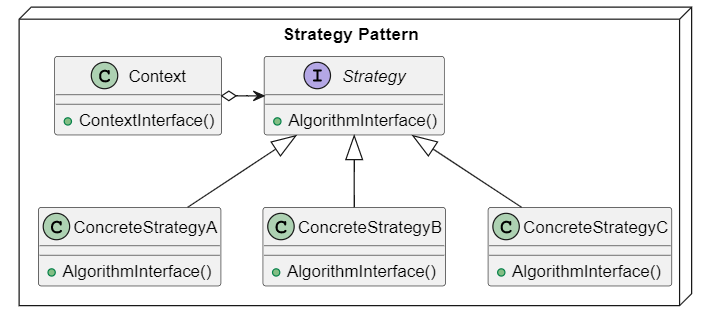
\includegraphics[width=0.6\linewidth]{UMLStrategyPattern}
     \caption{Strategie Pattern Struktur \cite{DesignPatterns}}
    \label{fig:StrategyPattern}
    \end{figure}
\end{center}
\vspace{-2cm}
Das Design Pattern besteht aus den folgenden Teilnehmern. Die \textit{Strategy}, welche eine gemeinsame Schnittstelle für die verwendeten Algorithmen deklariert. Einer oder mehreren \textit{ConcreteStrategy}, welche die Implementierung der Algorithmen oder Klassen ist, so wie dem \textit{Context}, welcher mit einer \textit{ConcreteStrategy} ausgestattet wird. Des Weiteren besitzt der \textit{Context} eine Referenz auf das \textit{Strategy} Objekt.\cite[S.383 ff]{DesignPatterns}\\
Über den \textit{Context} kann anschließend zur Laufzeit des Programmes die benötigten \textit{ConcreteStrategy} geladen und ausgeführt werden. 
Ein konkretes Beispiel hierzu wird im Buch Head First Design Patterns \cite{HeadfirstDesignPatterns} behandelt, was den nutzen dieses Patterns nochmal verdeutlicht.